\documentclass[12pt,a4paper]{article}
\usepackage{fontspec}
\usepackage{polyglossia}
\setdefaultlanguage{portuguese}
\usepackage{amsmath,amssymb}
\usepackage{graphicx}
\usepackage{booktabs}
\usepackage{multirow}
\usepackage{hyperref}
\usepackage{listings}
\usepackage{xcolor}
\usepackage{geometry}
\usepackage{float}
\usepackage{caption}
\usepackage{subcaption}

\geometry{margin=2.5cm}

\hypersetup{
    colorlinks=true,
    linkcolor=blue,
    filecolor=magenta,
    urlcolor=cyan,
}

\title{MAC0508 -- Introdução ao Processamento de Língua Natural\\
\vspace{0.5cm}
\Large EP2}

\author{Leonardo Heidi Almeida Murakami \\ NUSP:11260186}
\date{\today}

\begin{document}

\maketitle

\begin{abstract}
Este trabalho apresenta a implementação, treinamento e avaliação de modelos de tradução automática neural entre as línguas Português e Tupi Antigo. Utilizamos o modelo NLLB-200 (No Language Left Behind) em dois regimes de aprendizado: \textit{zero-shot}, onde o modelo é utilizado diretamente sem \textit{fine-tuning}, e \textit{few-shot}, onde realizamos o realizamos com o córpus disponível. Os resultados demonstram que o \textit{fine-tuning} melhora significativamente o desempenho, especialmente na direção Português$\rightarrow$Tupi Antigo, onde o BLEU aumentou de 5,52 para 27,52.
\end{abstract}

\section{Introdução}

Fazer tradução automática de línguas como o Tupi Antigo é um grande desafio para o Processamento de Língua Natural (PLN). Ao contrário de pares populares como inglês-portugues e portugues-inglês, para línguas indígenas como o Tupi Antigo existem poucos córpus paralelos, o que dificulta bastante o treinamento de modelos de tradução eficientes.

O Tupi Antigo foi a língua franca do Brasil colonial, utilizada amplamente pelos povos indígenas da costa brasileira e posteriormente adotada pelos colonizadores portugueses para comunicação com os nativos.

Este trabalho explora duas abordagens para tradução automática neste cenário de baixo recurso:

\begin{enumerate}
    \item \textbf{Zero-shot learning}: utilização direta de um modelo pré-treinado multilíngue, sem qualquer ajuste específico para o par linguístico em questão;
    \item \textbf{Few-shot learning via fine-tuning}: refinamento do modelo pré-treinado utilizando o córpus paralelo disponível.
\end{enumerate}

O objetivo é avaliar quantitativa e qualitativamente o desempenho de cada abordagem, utilizando métricas estabelecidas como BLEU e chrF, e identificar padrões de erro e acerto nas traduções produzidas.

\section{Descrição do Córpus}

\subsection{Origem dos Dados}

O córpus utilizado neste trabalho foi obtido do repositório público disponível em \url{https://github.com/CalebeRezende/oldtupi_dataset}. O arquivo original contém pares de sentenças em Português e Tupi Antigo, compilados a partir de fontes históricas e trabalhos de documentação linguística.

\subsection{Pré-processamento e Limpeza}

O processo de preparação do córpus envolveu as seguintes etapas:

\begin{enumerate}
    \item \textbf{Leitura do arquivo}: carregamento da planilha contendo as colunas ``PortuguÊs'' e ``Tupi Antigo'';
    \item \textbf{Limpeza textual}: remoção de caracteres especiais indesejados, normalização de espaços em branco, e eliminação de linhas vazias ou duplicadas;
    \item \textbf{Filtragem}: exclusão de pares onde qualquer uma das línguas estava ausente ou continha apenas espaços.
\end{enumerate}

\subsection{Estatísticas do Córpus}

Após o pré-processamento, o córpus final apresenta as seguintes características:

\begin{table}[H]
\centering
\caption{Estatísticas gerais do córpus}
\begin{tabular}{lc}
\toprule
\textbf{Métrica} & \textbf{Valor} \\
\midrule
Total de pares paralelos & 6.974 \\
\midrule
\multicolumn{2}{c}{\textit{Português}} \\
Média de caracteres por sentença & 35,7 \\
Média de palavras por sentença & 6,4 \\
\midrule
\multicolumn{2}{c}{\textit{Tupi Antigo}} \\
Média de caracteres por sentença & 26,2 \\
Média de palavras por sentença & 3,9 \\
\bottomrule
\end{tabular}
\label{tab:corpus_stats}
\end{table}

É legal de se notar que as sentenças em Tupi Antigo tendem a ser mais curtas, tanto em número de caracteres quanto de palavras, o que reflete características morfológicas da língua, como a aglutinação.

\subsection{Divisão do Córpus}

O córpus foi dividido em três subconjuntos, mantendo uma semente aleatória fixa (\texttt{random\_seed=42}) para reprodutibilidade:

\begin{table}[H]
\centering
\caption{Divisão do córpus em subconjuntos}
\begin{tabular}{lcc}
\toprule
\textbf{Subconjunto} & \textbf{Quantidade} & \textbf{Proporção} \\
\midrule
Treino & 4.881 & 70\% \\
Validação & 1.046 & 15\% \\
Teste & 1.047 & 15\% \\
\bottomrule
\end{tabular}
\label{tab:split}
\end{table}

O conjunto de teste é utilizado para avaliação em ambas as abordagens (zero-shot e few-shot), enquanto treino e validação são utilizados apenas no treinamento do few-shot.

\section{Metodologia}

\subsection{Seleção do Modelo}

Para este trabalho, selecionamos o modelo \textbf{NLLB-200-distilled-600M} (\textit{No Language Left Behind}), desenvolvido pela Meta AI. Esta escolha foi motivada pelos seguintes fatores:

\begin{enumerate}
    \item \textbf{Cobertura multilíngue}: o NLLB-200 foi treinado em 200 línguas, incluindo diversas línguas de baixo recurso, o que o torna adequado para generalização em cenários com dados limitados;
    
    \item \textbf{Arquitetura encoder-decoder}: baseado no Transformer, o modelo é especificamente projetado para tarefas de tradução sequência-a-sequência;
    
    \item \textbf{Suporte a línguas aparentadas}: embora o Tupi Antigo não esteja diretamente presente no vocabulário do modelo, utilizamos o código de língua do Guarani (\texttt{grn\_Latn}) como proxy, dado que ambas pertencem à família linguística Tupi-Guarani e compartilham características morfológicas e lexicais significativas;
    
    \item \textbf{Tamanho compacto}: a versão distilada com 600M de parâmetros permite \textit{fine-tuning} eficiente em hardware com recursos limitados.
\end{enumerate}

\subsection{Ambiente e Bibliotecas}

Para a implementação deste projeto, utilizamos Python 3.10+ com as seguintes bibliotecas principais:

\begin{itemize}
    \item \textbf{Transformers} (HuggingFace): biblioteca central para carregar e utilizar modelos pré-treinados. O modelo NLLB-200 é carregado diretamente do HuggingFace Hub através das classes \texttt{AutoModelForSeq2SeqLM} e \texttt{AutoTokenizer}
    
    \item \textbf{PyTorch}: framework de deep learning utilizado como backend para os modelos. Permite aceleração via GPU (CUDA) para treinamento e inferência
    
    \item \textbf{Datasets} (HuggingFace): gerenciamento eficiente de conjuntos de dados para treinamento
    
    \item \textbf{SacreBLEU}: implementação padronizada das métricas BLEU e chrF para avaliação
    
    \item \textbf{Accelerate}: otimização automática do treinamento para diferentes configurações de hardware
    
    \item \textbf{Pandas/NumPy}: manipulação e análise de dados.
\end{itemize}

O carregamento do modelo é feito de forma simples através da API do HuggingFace:

\begin{verbatim}
from transformers import AutoModelForSeq2SeqLM, AutoTokenizer

model_name = "facebook/nllb-200-distilled-600M"
tokenizer = AutoTokenizer.from_pretrained(model_name)
model = AutoModelForSeq2SeqLM.from_pretrained(model_name)
\end{verbatim}

Para o treinamento (\textit{fine-tuning}), utilizamos o \texttt{Seq2SeqTrainer} da biblioteca Transformers, que abstrai o loop de treinamento e oferece funcionalidades como checkpointing, logging e early stopping de forma integrada.

\subsection{Implementação Zero-shot}

Na abordagem zero-shot, o modelo NLLB é utilizado diretamente, sem qualquer ajuste adicional. O procedimento consiste em:

\begin{enumerate}
    \item Carregar o modelo pré-treinado e o tokenizador correspondente;
    \item Configurar os códigos de língua de origem e destino:
    \begin{itemize}
        \item Português: \texttt{por\_Latn}
        \item Tupi Antigo (via Guarani): \texttt{grn\_Latn}
    \end{itemize}
    \item Para cada sentença do conjunto de teste, gerar a tradução utilizando o método \texttt{generate} do modelo;
    \item Coletar as traduções e calcular as métricas de avaliação.
\end{enumerate}

A hipótese subjacente é que, devido ao treinamento massivo em múltiplas línguas, incluindo o Guarani (língua aparentada ao Tupi Antigo), o modelo pode apresentar capacidade de transferência para o Tupi Antigo mesmo sem treinamento específico.

\subsection{Implementação Few-shot com Fine-tuning}

Na abordagem few-shot, realizamos o refnamento do modelo NLLB utilizando o córpus de treinamento disponível. Os principais componentes desta implementação são:

\subsubsection{Configuração de Treinamento}

\begin{table}[H]
\centering
\caption{Hiperparâmetros de treinamento}
\begin{tabular}{lc}
\toprule
\textbf{Parâmetro} & \textbf{Valor} \\
\midrule
Tamanho do batch & 4 \\
Taxa de aprendizado & $5 \times 10^{-5}$ \\
Número máximo de épocas & 30 \\
Paciência (early stopping) & 5 épocas \\
Otimizador & AdamW \\
Warmup steps & 500 \\
Weight decay & 0,01 \\
\bottomrule
\end{tabular}
\label{tab:hyperparams}
\end{table}

\subsubsection{Early Stopping}

Para evitar \textit{overfitting}, implementamos um criterio de \textit{early stopping} baseado na perda de validação. O treinamento é interrompido se a perda de validação não melhorar por 5 épocas consecutivas, e o melhor checkpoint é restaurado.

\subsubsection{Treinamento Bidirecional}

Dois modelos separados foram treinados:
\begin{itemize}
    \item \textbf{PT$\rightarrow$TA}: tradução do Português para o Tupi Antigo
    \item \textbf{TA$\rightarrow$PT}: tradução do Tupi Antigo para o Português
\end{itemize}

\subsection{Métricas de Avaliação}

\subsubsection{BLEU (Bilingual Evaluation Understudy)}

A métrica BLEU avalia a qualidade da tradução através da sobreposição de n-gramas entre a tradução candidata e a referência. Utilizamos a implementação padrão com $n \leq 4$ e pesos uniformes ($w_1 = w_2 = w_3 = w_4 = 0,25$).

A pontuação BLEU varia de 0 a 100, onde valores mais altos indicam maior similaridade com a referência.

\subsubsection{chrF (CHaRacter-level F-score)}

A métrica chrF calcula a similaridade baseada em n-gramas de caracteres, sendo particularmente adequada para línguas com morfologia rica como o Tupi Antigo. Utilizamos duas variantes:

\begin{itemize}
    \item \textbf{chrF1} ($\beta = 1$): precisão e cobertura com igual importância
    \item \textbf{chrF3} ($\beta = 3$): cobertura com 3× mais importância que precisão
\end{itemize}

\section{Análise dos Resultados}

\subsection{Métricas Automáticas}

A Tabela~\ref{tab:results} apresenta os resultados comparativos entre as abordagens zero-shot e few-shot para ambas as direções de tradução.

\begin{table}[H]
\centering
\caption{Resultados comparativos das métricas de avaliação}
\begin{tabular}{llccc}
\toprule
\textbf{Experimento} & \textbf{Direção} & \textbf{BLEU} & \textbf{chrF1} & \textbf{chrF3} \\
\midrule
Zero-shot & PT$\rightarrow$TA & 5,52 & 13,43 & 16,75 \\
Few-shot & PT$\rightarrow$TA & \textbf{27,52} & \textbf{32,83} & \textbf{42,10} \\
\midrule
Zero-shot & TA$\rightarrow$PT & 45,18 & 30,53 & 22,15 \\
Few-shot & TA$\rightarrow$PT & \textbf{50,00} & \textbf{49,12} & \textbf{50,63} \\
\bottomrule
\end{tabular}
\label{tab:results}
\end{table}

\begin{figure}[H]
\centering
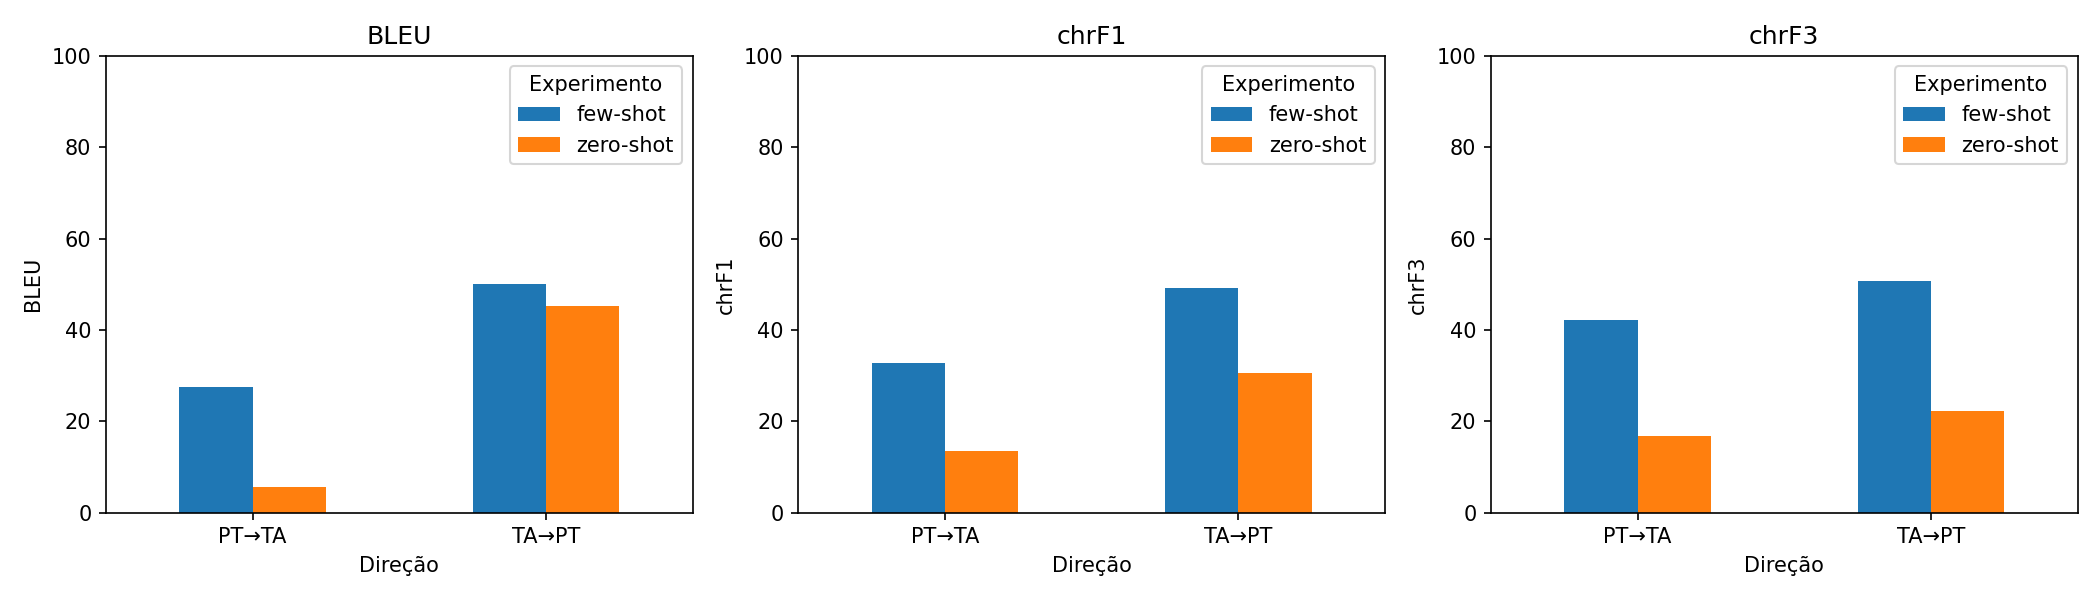
\includegraphics[width=\textwidth]{code/results/metrics_comparison.png}
\caption{Comparação visual das métricas entre experimentos}
\label{fig:metrics}
\end{figure}

\subsection{Análise por Direção de Tradução}

\subsubsection{Português $\rightarrow$ Tupi Antigo}

Esta direção apresenta o maior desafio, como evidenciado pelos resultados:

\begin{itemize}
    \item \textbf{Zero-shot}: BLEU de apenas 5,52 indica que o modelo praticamente não consegue produzir traduções adequadas sem treinamento específico. Isso era esperado, dado que o Tupi Antigo não está presente no vocabulário do modelo, e o Guarani moderno (usado como proxy) diverge significativamente;
    
    \item \textbf{Few-shot}: O \textit{fine-tuning} proporciona uma melhoria significante no BLEU (de 5,52 para 27,52), demonstrando que mesmo com um córpus relativamente pequeno, o modelo consegue aprender padrões significativos da língua alvo.
\end{itemize}

\subsubsection{Tupi Antigo $\rightarrow$ Português}

Esta direção apresenta desempenho consideravelmente melhor:

\begin{itemize}
    \item \textbf{Zero-shot}: BLEU de 45,18 é surpreendentemente alto, sugerindo que o modelo consegue extrair significado do Tupi Antigo e produzir traduções razoáveis em Português. Isso pode ser atribuído à maior familiaridade do modelo com o Português como língua alvo;
    
    \item \textbf{Few-shot}: Melhoria no BLEU (de 45,18 para 50,00), com ganhos mais expressivos em chrF1 (60,9\% de aumento) e chrF3 (128,6\% de aumento).
\end{itemize}

\section{Análise Linguística Qualitativa}

\subsection{Exemplos Positivos -- Zero-shot}

\subsubsection{PT$\rightarrow$TA}

\begin{table}[H]
\centering
\small
\begin{tabular}{p{3cm}p{4cm}p{4cm}c}
\toprule
\textbf{Fonte (PT)} & \textbf{Referência (TA)} & \textbf{Predição} & \textbf{BLEU} \\
\midrule
Quem és tu? & Abápe nde? & ¿Mávapa nde? & 55,0 \\
tuas palavras & nde nhe'enga & nde ñe'ẽnguéra & 50,0 \\
Preparai-vos! & Peîemosako'i! & Peñembosako'i! & 50,0 \\
\bottomrule
\end{tabular}
\caption{Melhores traduções zero-shot PT$\rightarrow$TA}
\end{table}

Observa-se que o modelo consegue capturar estruturas básicas como pronomes possessivos (\textit{nde}), mesmo sem treinamento específico, uma caracteristica que provavelmente se manteve do Tupi Antigo para o Guarani Moderno.

\subsubsection{TA$\rightarrow$PT}

\begin{table}[H]
\centering
\small
\begin{tabular}{p{4cm}p{4cm}p{4cm}c}
\toprule
\textbf{Fonte (TA)} & \textbf{Referência (PT)} & \textbf{Predição} & \textbf{BLEU} \\
\midrule
Salve Rainha, moraûsubara sy & Salve Rainha, mãe de misericórdia & Salve Rainha, mãe de moraúsubara & 76,0 \\
Tupã sy-porangeté & Mãe de Deus muito bela & Mãe de Deus & 51,3 \\
Peîemosako'i! & Preparai-vos! & Preparem-se! & 50,0 \\
\bottomrule
\end{tabular}
\caption{Melhores traduções zero-shot TA$\rightarrow$PT}
\end{table}

\subsection{Exemplos Positivos -- Few-shot}

\subsubsection{PT$\rightarrow$TA}

\begin{table}[H]
\centering
\small
\begin{tabular}{p{5cm}p{5cm}c}
\toprule
\textbf{Fonte (PT)} & \textbf{Referência = Predição (TA)} & \textbf{BLEU} \\
\midrule
Guardai-vos de serdes maus doravante & Peteumẽ pe poxyramo angiré & 100,0 \\
Caburé, vem correndo! & Kaburé, îori enhana! & 100,0 \\
Veio um grande chefe & Oú tubixá-katu & 100,0 \\
\bottomrule
\end{tabular}
\caption{Melhores traduções few-shot PT$\rightarrow$TA}
\end{table}

O modelo \textit{fine-tuned} consegue reproduzir traduções perfeitas para diversas sentenças, demonstrando aprendizado efetivo dos padrões linguísticos.

\subsubsection{TA$\rightarrow$PT}

\begin{table}[H]
\centering
\small
\begin{tabular}{p{4cm}p{5cm}c}
\toprule
\textbf{Fonte (TA)} & \textbf{Referência = Predição (PT)} & \textbf{BLEU} \\
\midrule
Xe pytaî turi & Veio atrás de mim & 100,0 \\
Pedro ranhẽ osó & Pedro foi primeiro & 100,0 \\
Xe îekyîme, t'ereîu & Quando eu morrer, que venhas & 100,0 \\
\bottomrule
\end{tabular}
\caption{Melhores traduções few-shot TA$\rightarrow$PT}
\end{table}

\subsection{Exemplos Negativos}

\subsubsection{Zero-shot}

\begin{table}[H]
\centering
\small
\begin{tabular}{p{3.5cm}p{3.5cm}p{4cm}}
\toprule
\textbf{Fonte} & \textbf{Referência} & \textbf{Predição (incorreta)} \\
\midrule
\multicolumn{3}{c}{\textit{PT$\rightarrow$TA}} \\
Estou de acordo com ele & Supi nhẽ aîkó & Añe'ẽ porã hese \\
Frustrei-me & Xe rambûer & Añeñandu vaieterei \\
\midrule
\multicolumn{3}{c}{\textit{TA$\rightarrow$PT}} \\
mby piru'a & calos dos pés & abóbora \\
Asa'ubar & Tomei-o em seco & Acasoubar \\
\bottomrule
\end{tabular}
\caption{Piores traduções zero-shot}
\end{table}

Os erros no modo zero-shot demonstram que o modelo frequentemente:
\begin{itemize}
    \item Produz traduções em Guarani moderno em vez de Tupi Antigo, o que faz sentido ja que é nossa seleção de entrada para o modelo;
    \item Falha em reconhecer vocabulário específico do Tupi Antigo;
\end{itemize}

\subsubsection{Few-shot}

\begin{table}[H]
\centering
\small
\begin{tabular}{p{3.5cm}p{3.5cm}p{4cm}}
\toprule
\textbf{Fonte} & \textbf{Referência} & \textbf{Predição (incorreta)} \\
\midrule
\multicolumn{3}{c}{\textit{PT$\rightarrow$TA}} \\
Eu sou melhor que tu & Xe katu-eté nde suí & Nde sosé ixé ipó \\
ovos de içá & ysá rupi'a & îyá ruba \\
\midrule
\multicolumn{3}{c}{\textit{TA$\rightarrow$PT}} \\
Aporoîuká & Mato gente & Matá-lo-ei \\
Xe moapysy-katu & Deleita-me muito & Afligiu-me muitíssimo \\
\bottomrule
\end{tabular}
\caption{Piores traduções few-shot}
\end{table}

Mesmo após o \textit{fine-tuning}, o modelo ainda apresenta dificuldades com:
\begin{itemize}
    \item Estruturas comparativas;
    \item Vocabulário especializado (fauna, flora, partes do corpo);
    \item Inversão de polaridade semântica (deleitar vs. afligir).
\end{itemize}

\section{Conclusões e Limitações}

\subsection{Conclusões}

Este trabalho demonstrou a viabilidade de utilizar modelos de linguagem pré-treinados para tradução automática de línguas de baixo recurso, especificamente o par Português--Tupi Antigo.

Os principais achados são:

\begin{enumerate}
    \item O \textit{fine-tuning} proporciona melhorias substanciais em relação ao modo zero-shot, especialmente na direção PT$\rightarrow$TA (aumento de 398\% no BLEU);
    
    \item A tradução TA$\rightarrow$PT é consideravelmente mais fácil, provavelmente devido à maior familiaridade do modelo com o Português como língua alvo;
    
    \item A utilização do Guarani como proxy para o Tupi Antigo é uma estratégia válida, mas com limitações evidentes no vocabulário e estruturas específicas;
    
    \item Mesmo com um córpus relativamente pequeno (4.881 pares de treino), foi possível alcançar traduções perfeitas (BLEU = 100) para diversas sentenças.
\end{enumerate}

\subsection{Limitações}

\begin{enumerate}
    \item \textbf{Tamanho do córpus}: com menos de 7.000 pares, o modelo não consegue aprender a diversidade completa da língua;
    
    \item \textbf{Proxy linguístico}: o uso do Guarani como substituto para o Tupi Antigo introduz ruído, especialmente em vocabulário específico;
    
    \item \textbf{Variação ortográfica}: textos históricos apresentam variação ortográfica que pode confundir o modelo;
\end{enumerate}

\end{document}

